\message{ !name(main.tex)}%
% Choose how your presentation looks.
\documentclass{beamer}

% For more themes, color themes and font themes, see:
% http://deic.uab.es/~iblanes/beamer_gallery/index_by_theme.html
%
\mode<presentation>
{
  \usetheme{default}      % or try Darmstadt, Madrid, Warsaw, ...
  \usecolortheme{default} % or try albatross, beaver, crane, ...
  \usefonttheme{default}  % or try serif, structurebold, ...
  \setbeamertemplate{navigation symbols}{}
  \setbeamertemplate{caption}[numbered]
}

\usepackage[english]{babel}
\usepackage[utf8x]{inputenc}
\usepackage{graphicx}
\usepackage{natbib}
\usepackage{subcaption}
\usepackage{mathtools}
\usepackage{nicefrac} % compact symbols for 1/2, etc.
\usepackage{microtype} % microtypography
\usepackage{lipsum}
\usepackage{physics}
\usepackage{amsmath}
\usepackage{amssymb}
\usepackage{booktabs}
\usepackage{cancel}


\newcommand{\mc}[1]{\mathcal{#1}}
\newcommand{\bolds}[1]{\boldsymbol{#1}}
% \DeclarePairedDelimiter\abs{\lvert}{\rvert}%

%1 Exectation value
\newcommand{\expect}[1]{\langle{}{#1}\rangle{}}

% Collections of samples
\newcommand{\mcH}{\mathcal{H}}
\newcommand{\mcE}{\mathcal{E}}
\newcommand{\mcB}{\mathcal{B}}
\newcommand{\mcV}{\mathcal{V}}
\newcommand{\mcX}{\mathcal{X}}
\newcommand{\mcY}{\mathcal{Y}}
\newcommand{\mcC}{\mathcal{C}}
\newcommand{\mcS}{\mathcal{S}}
\newcommand{\mcL}{\mathcal{L}}
\newcommand{\mcR}{\mathcal{R}}


% Microstates (bold lowercase)
\newcommand{\bh}{\bolds{h}}
\newcommand{\be}{\bolds{e}}
\newcommand{\bb}{\bolds{b}}
\newcommand{\bv}{\bolds{v}}
\newcommand{\bx}{\bolds{x}}
\newcommand{\by}{\bolds{y}}
\newcommand{\bs}{\bolds{s}}
\newcommand{\bo}{\bolds{o}}
\newcommand{\br}{\bolds{r}}

% Microstates (bold lowercase)
\newcommand{\bH}{\bolds{H}}
\newcommand{\bE}{\bolds{E}}
\newcommand{\bB}{\bolds{B}}
\newcommand{\bV}{\bolds{V}}
\newcommand{\bX}{\bolds{X}}
\newcommand{\bY}{\bolds{Y}}
\newcommand{\bS}{\bolds{S}}
\newcommand{\bT}{\bolds{T}}

% microstates explicit (bold lowercase)
\newcommand{\seth}{\{h_j\}}
\newcommand{\sete}{\{e\}}
\newcommand{\setb}{\{b\}}
\newcommand{\setv}{\{v_i\}}
\newcommand{\setx}{\{x_i\}}
\newcommand{\sety}{\{y_j\}}
\newcommand{\sets}{\{s_i\}}
\newcommand{\setr}{\{r_j\}}

\DeclareMathOperator*{\argmin}{argmin}
\DeclareMathOperator{\sgn}{sgn}

% Greek letters
\renewcommand{\l}{\lambda}
\renewcommand{\b}{\beta}
\renewcommand{\L}{\Lambda}
\renewcommand{\k}{\kappa}
\newcommand{\T}{\Theta}
\renewcommand{\P}{\Psi}


\title[RBMs and RG: Learning Relevant Information]{Restricted Boltzmann Machines and the Renormalization Group: Learning Relevant Information in Statistical Physics}

\author{Jesse Hoogland}
\institute{Amsterdam University College}

\date{05-06-2019}

% BEGIN DOCUMENT

\begin{document}

\message{ !name(main.tex) !offset(-3) }


\begin{frame}
  \titlepage
\end{frame}

\section{Introduction}
\begin{frame}{Introduction}
  \begin{itemize}
  \item The Renormalization Group (RG) of Statistical Physics
  \item Deep Neural Networks (DNNs) in Machine Learning
  \item Information and Probability Theory
  \end{itemize}
\end{frame}


\begin{frame}{Outline}
  \tableofcontents
\end{frame}

\section{Statistical Physics}

% Let us start at the beginning, with the origins of statistical physics
% Thermodynamics -> SP
% Need for explanation of heat: continuous wave-like or discrete and atomic
% The latter
% Controversial - need to defend theories with experimental predictions
% GOAL: TRANSLATING MICRO TO MACRO

\begin{frame}{Introduction to Statistical Physics}
  \begin{figure}[h!]
    \centering
    \begin{subfigure}[b]{0.25\linewidth}
      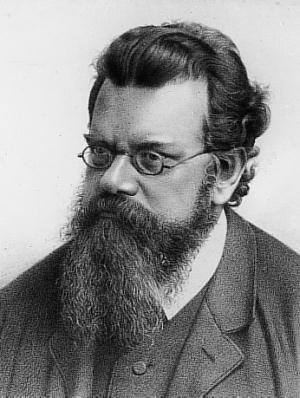
\includegraphics[width=\linewidth]{figures/boltzmann.jpeg}
      \caption{Ludwig Boltzmann~\cite{boltzmann}}
    \end{subfigure}%
    \quad
  \begin{subfigure}[b]{0.25\linewidth}
    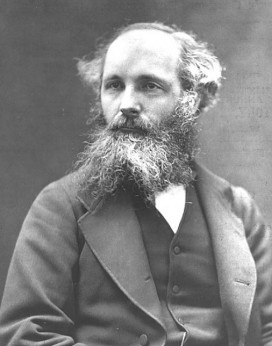
\includegraphics[width=\linewidth]{figures/maxwell.jpeg}
    \caption{James Clerk Maxwell~\cite{maxwell}}
  \end{subfigure}%
\quad
  \begin{subfigure}[b]{0.25\linewidth}
    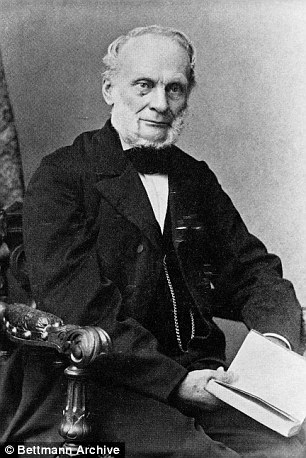
\includegraphics[width=\linewidth]{figures/clausius.jpeg}
    \caption{Rudolf Clausius~\cite{clausius}}
  \end{subfigure}
  \label{fig:the-greats}
\end{figure}
\end{frame}

% Anchor our investigation in one specific example: FERROMAGNETISM
% Our goal will be to predict properties of these magnets.
% PIVOT: what kinds of predictions can we make?
\section{Ferromagnetism}
\begin{frame}{Ferromagnetism}
  \begin{figure}[ht]
    \centering
    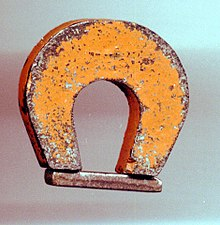
\includegraphics[width=0.5\linewidth]{figures/magnet.jpg}
    \caption{Ferromagnetism, the process by which materials like iron form permanent magnets.\label{fig:label} }
  \end{figure}
\end{frame}

% Specifically, if we control the temperature and an external field,
% What will we MEASURE:
%    - Magnetization, Susceptibility, Specific heat, etc.

\subsection{Macroparameters}
\begin{frame}{Macroparameters}
  \begin{tabular}{ll}
    \toprule
    Macroparameter & Description\\
    \midrule
    Magnetization. & The strength of the magnet's field.\\
    Spontaneous magnetization & Magnetization even\\
                   &in the absence of an external magnetic field.\\
    Zero-field susceptibility & How much the \\
                   &magnetization changes for small changes in temperature.\\
    Specific heat & How much the average \\
                   &energy changes for small changes in temperature.\\
    \bottomrule
  \end{tabular}
\end{frame}

% We have to be a bit more precise with what we mean by MEASUREMENT
% MICROSTATE - how the atoms are configured and vibrating etc.
% In square cm of air - million million million molecules
% No way to measure the microstate exactly (QM and Practical, data limits, etc)
% System is updating rapidly
% What we end up measure

\subsection{Measurements as Expectations}
\begin{frame}{Measurements as Averages}
  \begin{equation}%
   \boxed{ \expect{M}\:=\sum_{\bs\in\mcS} P(\bs) M(\bs)\label{eq:expectation-as-average}}
  \end{equation}
\end{frame}

% FUNDAMENTAL ASSUMPTION OF SM
% Clever reasaoning we can get to the boltzmann distribution
% For systems that exchange only energy to their surroundings,
% Probability is related to energy. More energy = less likely
% FUNDAMENTAL PROBLEM OF SM: Intractable Z. However Z also very useful.
% PIVOT: Returning to our magnet, let's try an devise a suile energy model.
%        It turns out, the simplest we can do is the Ising model.
\subsection{The Boltzmann Distribution}
\begin{frame}{The Boltzmann Distribution}
  \begin{equation}%
    \boxed{P(\bs)\:=\frac{1}{Z}e^{-\b E(\bs)}\quad Z\:=\sum_{\bs} e^{-\b E(\bs)}}\label{eq:boltzmann-distribution}
  \end{equation}%
\end{frame}
% PIVOT: To solve for probabilities and expectation vlaues we need energies
\subsection{The Ising Model}
\begin{frame}{The Ising Model}
  \begin{equation}%
    \bs = \left(
      \begin{pmatrix}
        s_1\\
        s_2\\
        \vdots\\
        s_N
      \end{pmatrix}
    \right)
  \end{equation}%

  \begin{equation}%
    s_i\in\{-1,1\}
  \end{equation}%

  \begin{equation}%
    M(\bs)=\sum_i s_i
  \end{equation}%

  \begin{figure}[ht]
    \centering
    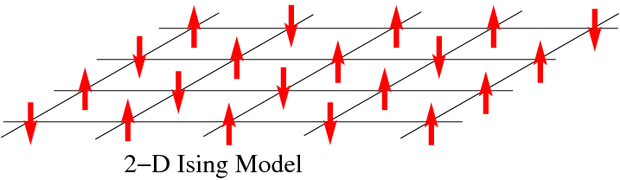
\includegraphics[width=0.5\textwidth]{figures/ising.png}
    \caption{The Ising model~\cite{ising}.\label{fig:ising} }
  \end{figure}

\end{frame}

% You can actually solve the Boltzmann distribution for this energy
% function in 1 and 2 dimensions 3 - proven to be NP-Hard PIVOT:
% Instead of solving these exactly, we'll consider approximate methods
% More representative of real-life investigations
\section{The Ising Hamiltonian}
\begin{frame}{The Ising Hamiltonian}
  \begin{equation}
    \boxed{E(\bs)\:= -B \sum_i s_i-J \sum_{\langle i,j\rangle} s_i s_j}
    \label{eq:ising-energy}
  \end{equation}%

  \begin{enumerate}
  \item $B$: The external magnetic field.
  \item $J$: The interaction strength between neighboring spins.
  \end{enumerate}
\end{frame}

%
\begin{frame}{Markov-Chain Monte Carlo (MCMC) Methods}
  \begin{itemize}
  \item Perform ensemble average over a subset of (representative)
    samples.
  \item Relative probabilities are easier to evaluate than absolute
    probabilities.
  \end{itemize}

   \begin{equation}%
     \boxed{P(\bs)\:=\frac{1}{Z}e^{-\b E(\bs)}\quad Z\:=\sum_{\bs} e^{-\b E(\bs)}}
   \end{equation}%

\begin{figure}[ht]
  \centering 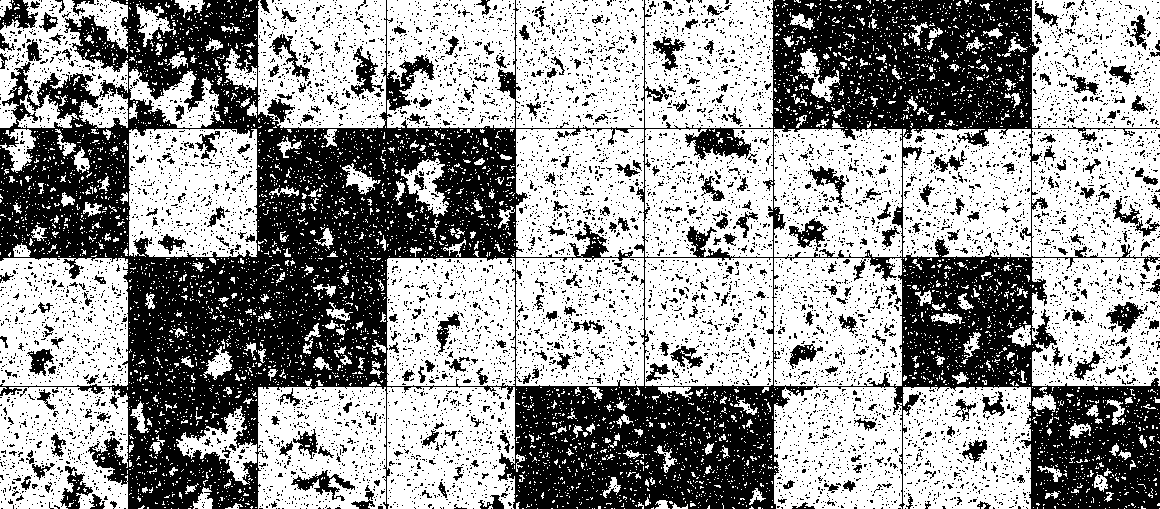
\includegraphics[width=\textwidth]{figures/samples.png}
\end{figure}

\end{frame}

\begin{frame}{Mean-Field Theory (MFT)}
  \begin{itemize}
  \item Approximate the value at each spin by an average over its
    neighbors.
  \item Gives some really interesting predictions about
    \textit{critical behavior}.
  \end{itemize}

\begin{figure}[ht]
  \centering
  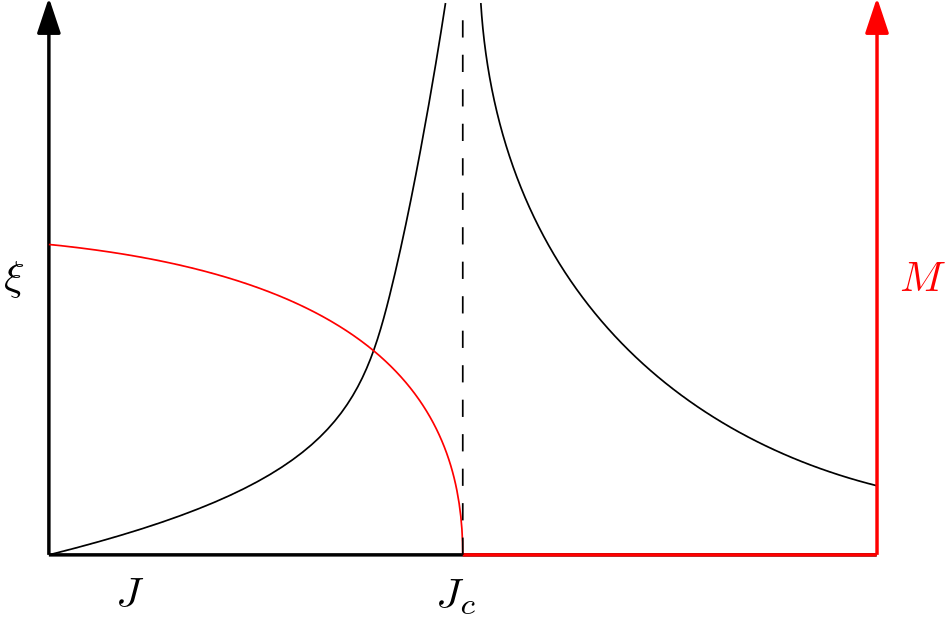
\includegraphics[width=.5\textwidth]{figures/correlation-length.png}
  \caption{MFT predicts a \textit{critical point}, below which the
    system \textit{spontaneously magnetizes}. At the critical point,
    MFT predicts a divergence of the correlation length.}
\end{figure}
\end{frame}

% PIVOT: However, these are WRONG
\begin{frame}{Mean-Field Theory Critical Exponents}
  \begin{equation}%
    \boxed{\expect{M}\rvert_{B=0}\sim\abs{t}^{-1/2}}
  \end{equation}%
  \begin{equation}%
    \xi\sim\abs{t}^{-1/2}
\end{equation}%

$t$ is the \textit{reduced temperature}: $t:=(T-T_c)/T_c$.
\end{frame}

% PIVOT: we need something else to make quantitative predictions
\begin{frame}{Mean-Field Theory Critical Exponents}
  \begin{equation}%
    \boxed{\expect{M}\rvert_{B=0}\xcancel{\sim}\abs{t}^{-1/2}}
  \end{equation}%
  \begin{equation}%
    \xi\xcancel{\sim}\abs{t}^{-1/2}
\end{equation}%
$t$ is the \textit{reduced temperature}: $t:=(T-T_c)/T_c$.
\end{frame}

\section{The Renormalization Group}
\begin{frame}{The Renormalization Group}
Instead of computing $Z=\sum_{\bs}e^{-\b E(\bs)}$ explicitly, try to reexpress $Z$ in a simpler form.
\begin{equation}%
\boxed{\sum_{\bs'}e^{-H'(\bs')}=\sum_{\bs}e^{-H(\bs)}}
\end{equation}%

For example, \textit{decimation}:
\begin{equation}%
  e^{-H'(\bs')}=\sum_{s_2,s_4,\ldots,s_N} e^{-H(\bs)},
\end{equation}%
\end{frame}

% We can do this for any one microstate easily, but as we saw from (go back),
% we need to perform this sum for ALL microstates. STILL INTRACTABLE
% PIVOT:
\subsection{Majority-Rule Block-Spin Renormalization}
\begin{frame}{Majority-Rule Block-Spin Renormalization}
  \begin{enumerate}
  \item Divide configuration into $j$ (3x3) ``blocks,''
    $\bv^{(j)}=(v_1^{(j)},\cdot, v_9^{(j)})$).
  \item For each block, create a new \textit{coarse-grained} spin
    $h_j$, according to the \textit{majority-rule}:
    \begin{equation}%
      \boxed{h_j=\sgn \sum_{i=1}^9 v_i}
    \end{equation}%
  \item Rescale our coarse-grained configuration to the original block
    size.
  \end{enumerate}

\begin{figure}[ht]
  \centering
  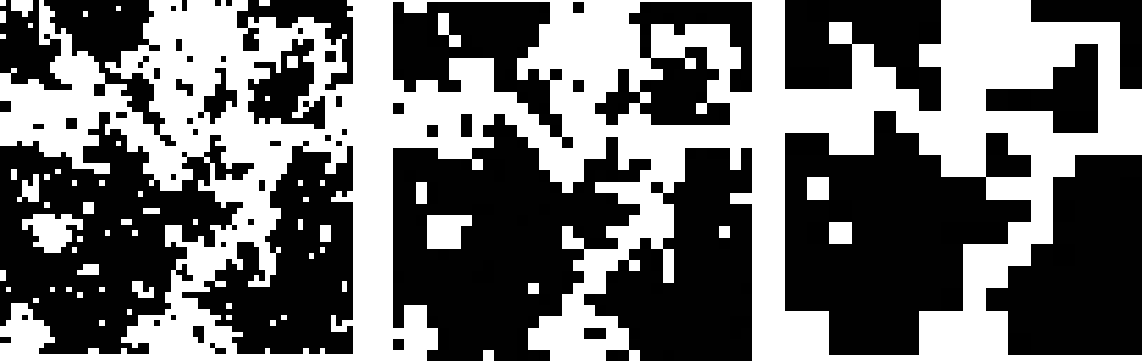
\includegraphics[width=.5\textwidth]{figures/block-rg.png}
  \caption{Three steps of majority-rule block-spin renormalization,
    preceding left to right (block size $b=2$).\label{fig:block-rg} }
\end{figure}

\end{frame}

% TURNS OUT THIS IS NOT ENTIRELY ACCURATE

\begin{frame}{Working out the details}
  Suppose $J' = \mathcal{R}(J)$, then a critical point is such that
  $J^* =\mathcal{R}(J^*)$.  In its vicinity:
  \begin{equation}
    J'\approx \mathcal{R}(J^*)+ \mathcal{R}'(J^*)(J-J^*) = J^* + b^y(J-J^*),
  \end{equation}
  where $b$ is the block size and
  \begin{equation}
    y \equiv \frac{\ln{\mathcal{R}'(J^*)}}{\ln{b}}.
  \end{equation}

  Knowing that
  \begin{equation}
    \xi(J) \sim A (J-J^*)^{-\nu},
  \end{equation}
  we determine:
  \begin{equation}%
    \boxed{\nu=\frac{1}{y_t}}
  \end{equation}%
\end{frame}

\begin{frame}{Relevant Operators}
  \begin{equation}%
  \boxed{y\rightarrow y_i}
  \end{equation}%
\begin{itemize}
\item $y_i > 0$: \textbf{relevant}, repeated RG iterations bring us away from fixed point value.
\item $y_i < 0$: \textbf{irrelevant}, repeated RG iterations bring us closer to fixed point value.
\item $y_i = 0$: \textbf{marginal}, linearized equations do not provide enough information.
\end{itemize}
\end{frame}

\begin{frame}{Consequences of RG}
  \begin{itemize}
  \item \textit{RG-flow}: Critical exponents are expressed as derivatives of RG
    transformations.
  \item \textit{Scaling relations}: we can express critical exponents in terms of one another.
  \item \textit{Universality}: there are finitely many fixed points,
    and many microscopic theories are indistinguishable
    macroscopically.
  \end{itemize}
\end{frame}

\begin{frame}{RG in Practice}
\begin{itemize}
\item $4-\epsilon$ expansion.
\item MCMC methods and finite-size scaling.
\item Kadanoff's method $e^{-H'(s')}=\sum_s e^{\bT_\l(s',s)-H(s)}$.
\end{itemize}
\end{frame}

\section{Machine Learning}
\begin{frame}{Partition Functions or Probability Distributions}
  \textem{Statistical Physics}
  \begin{align}%
    H(\bs)\rightarrow Z &\rightarrow \mcS\\
    \frac{P(\bs)}{P(\bs')}&\rightarrow \mcS_{data}
  \end{align}%

  \textem{Machine Learning}
  \begin{align}%
    \mcS&\rightarrow P_\\
    \mcS_{data}&\rightarrow P_{\theta}(\bs)
  \end{align}%

\end{frame}

\begin{frame}{Feed-Forward Neural Networks}
  \begin{figure}[ht]
    \centering 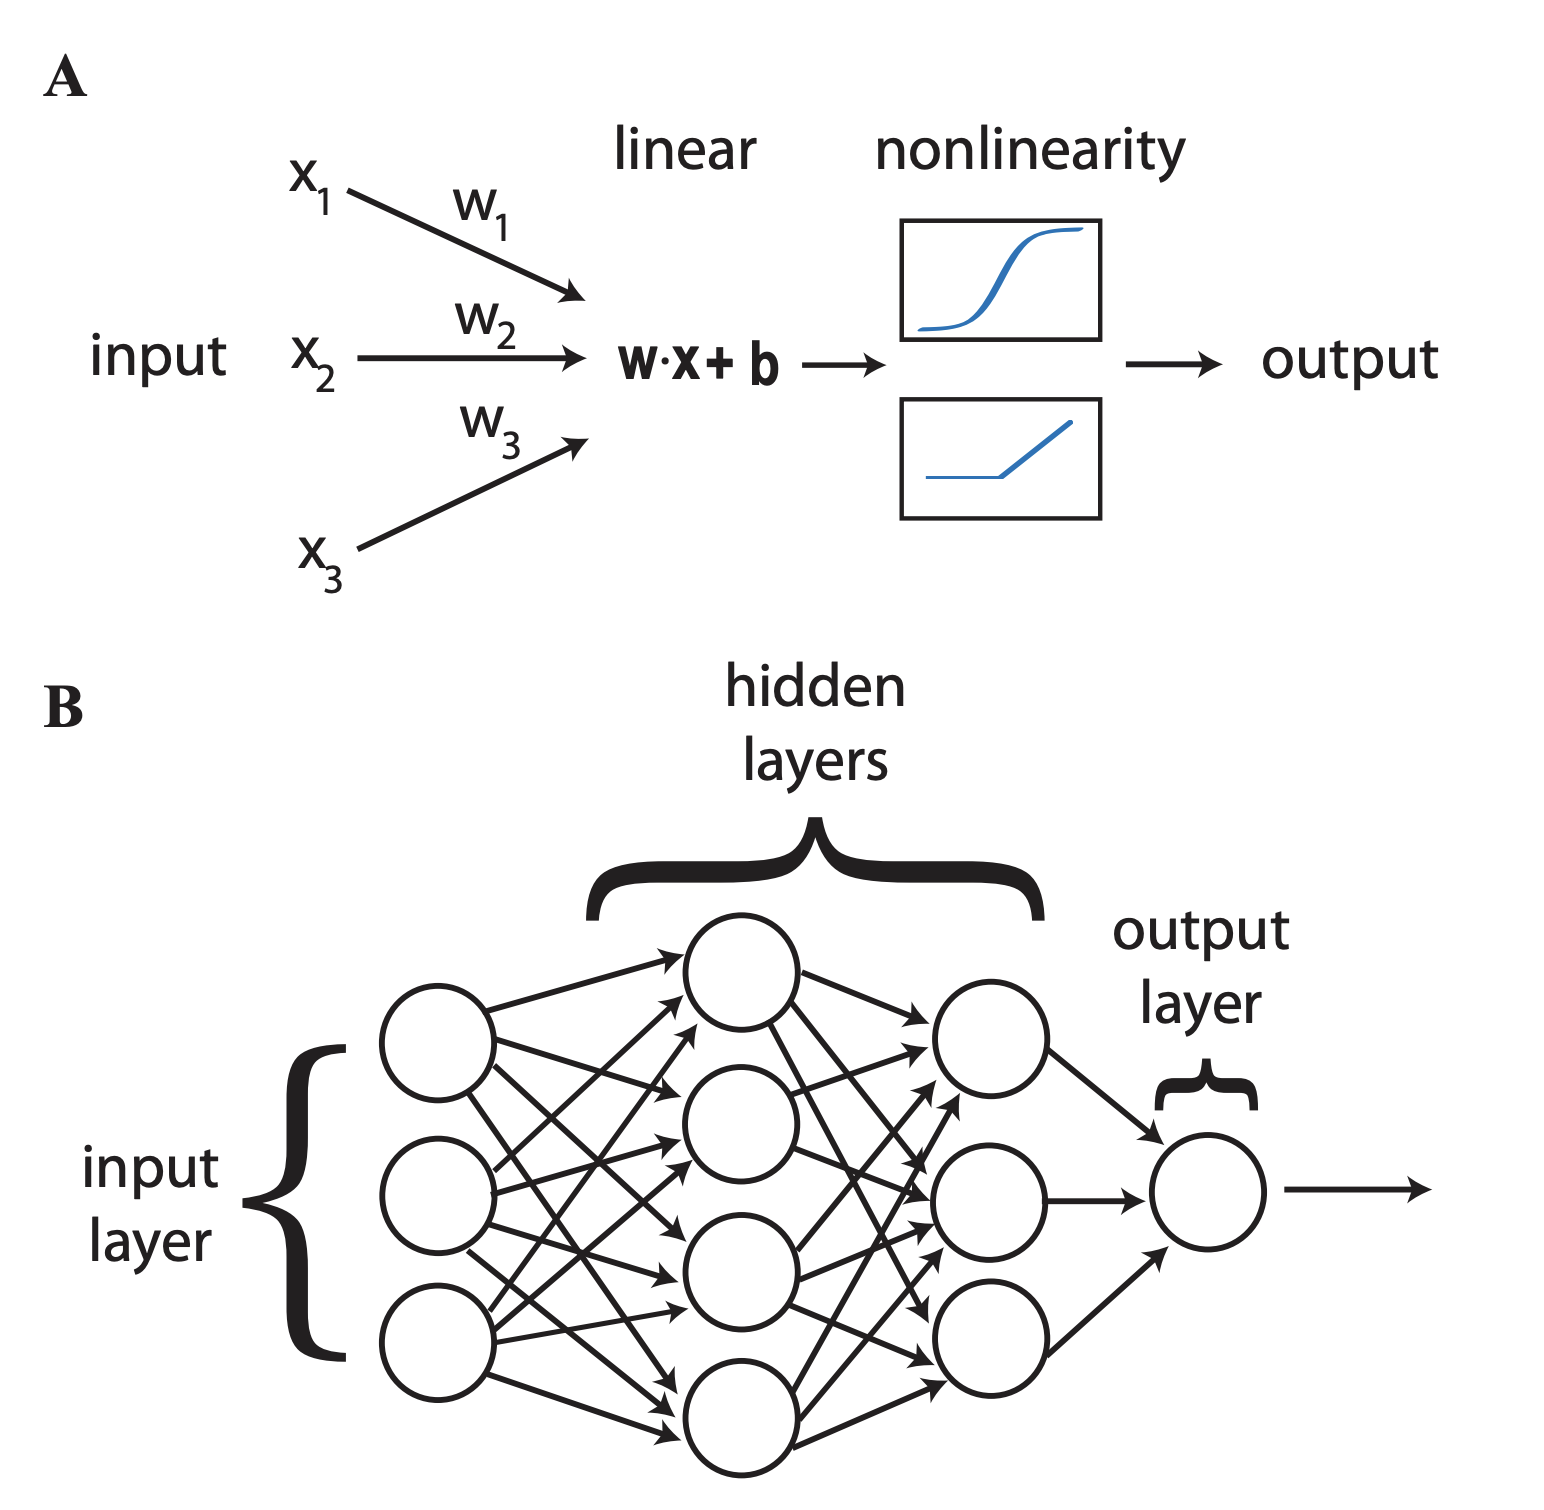
\includegraphics[width=0.7/linewidth]{figures/ffnn.png}
    \caption{A neural network consists of alternating linear and
      non-linear transformations.}
  \end{figure}

\end{frame}

\begin{frame}{Restricted Boltzmann Machines (RBMs)}
  \begin{figure}[ht]
    \centering 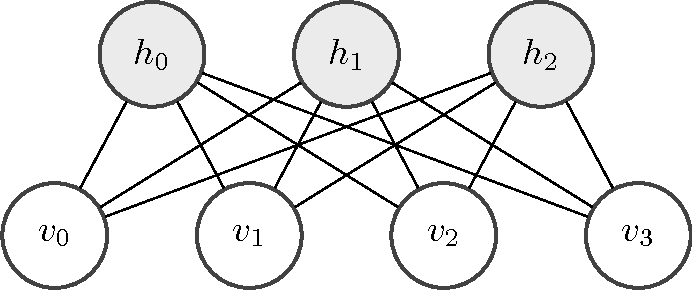
\includegraphics[width=0.7\linewidth]{figures/rbm.png}
    \caption{RBMs are a bidirectional neural network of binary-valued
      units.}
  \end{figure}
\end{frame}

\begin{frame}{RBM Probabilities}
  \begin{equation}%
    \boxed{E_\theta(\bv, \bh):=-\sum_i a_iv_i -\sum_j b_jh_j-\sum_{ij} w_{ij}v_ih_j \label{eq:rbm-energy-fn}}
  \end{equation}
  \begin{equation}%
    \boxed{P_\theta(\bv,\bh):=\frac{1}{Z}e^{-E_\theta(\bv,\bh)}\quad
      Z:=\sum_{\bv',\bh'}e^{E_\theta(\bv', \bh')}\label{eq:rbm-joint-dist}}
  \end{equation}%
\end{frame}

\begin{frame}{Phase Classifier}
  \begin{equation}
    \boxed{P_\theta(\bh|\bv)=\prod_{j=1}^M \frac{1}{1+e^{-h_j(\sum_i w_{ij} v_i +b_j )}}
    }\label{eq:v-to-h}
  \end{equation}%
  \begin{figure}[ht]
    \centering
    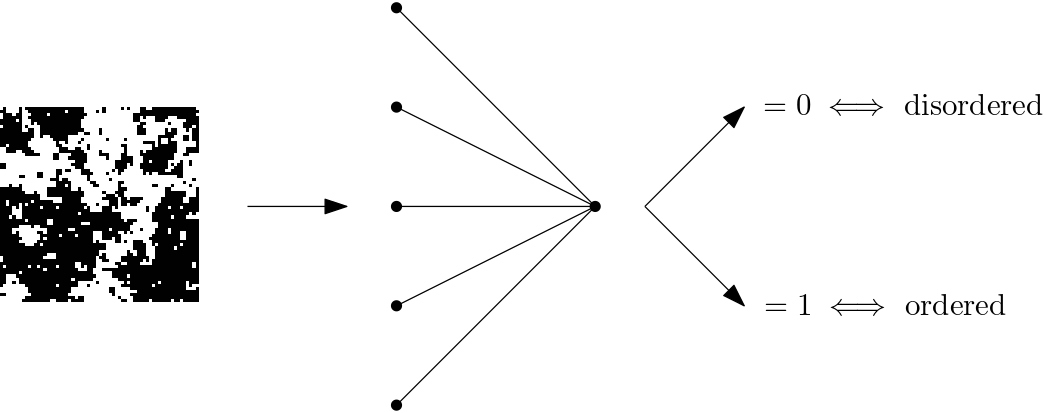
\includegraphics[height=0.5\lineheight]{figures/classifier.png}
    \caption{We can use $P_\theta(\bh\rvert\bv)$ as a phase
      classifer.}
  \end{figure}


\end{frame}

% COND PROBS instead of ABS PROBS
\begin{frame}{Gibbs Sampling}
  \begin{equation}%
    \boxed{P(\bv)=\sum_{\bh}P(\bv,\bh)}
  \end{equation}%

  \begin{figure}[ht]
    \centering
    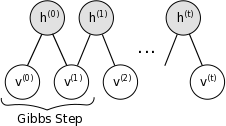
\includegraphics[width=0.5\linewidth]{figures/gibbs_steps.png}
    \caption{RBMs can implement a MCMC sampling technique known as
      \textit{Gibbs sampling}.}
  \end{figure}

\end{frame}

% Note qualitative similarities

\begin{frame}{RG = RBM?}
  \begin{figure}[ht]
    \centering
    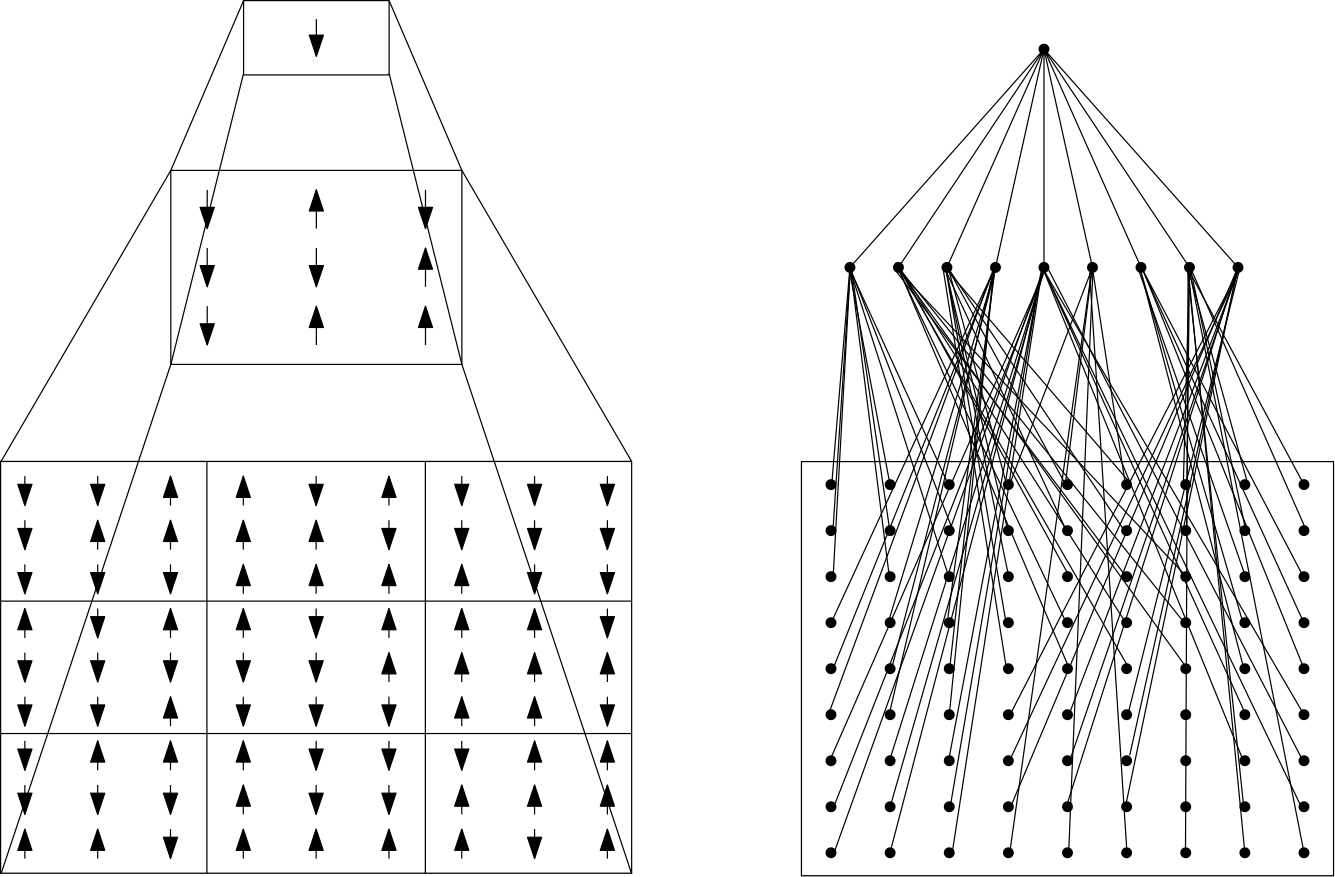
\includegraphics[width=0.5\textwidth]{figures/rg-rbm.png}
    \caption{Two iterations of block renormalization and a deep
      Boltzmann machine of three layers.\label{fig:rbm-rg} }
  \end{figure}
\end{frame}

\begin{frame}{Relevant Information}
  Relevant information is the information contained in one signal $x$
  about another $y$. This is quantified with the mutual information:%
  \begin{equation}%
    \boxed{I(\bx; \by)\eqcolon\sum_{\bx,\by}P(\bx,\by)\log\left(\frac{P(\bx,\by)}{P(\bx)P(\by)}\right)}
  \end{equation}%
\end{frame}


\begin{frame}{An Exact Correspondence between Kadanoff's Variational
    RG and RBMs}
\begin{equation}
  \bT_\l(\bv, \bh)=-\bolds{E}_\theta(\bv,\bh)+\bolds{H}(\bv),
\end{equation}
  \begin{equation}%
P_\theta(x)=P_{\text{true}}(x)=\iff Z'_{\text{Kadanoff}}=Z
  \end{equation}%
\end{frame}



\section{References}
\begin{frame}{References}
\bibliographystyle{unsrt} \bibliography{references}
\end{frame}

\end{document}

\message{ !name(main.tex) !offset(-528) }
